% !TEX root = C:\Users\Jan\Documents\dev\Risk-Measurement-Framework\masterthesis_tex\masterthesis_main.tex
\section{Risk results template}
\label{sec:template}

At first, the evaluated measurement shows the risk matrices. Figure \ref{fig:rm_template} shows such a risk matrix.

\begin{figure}[h!]
  \centering
  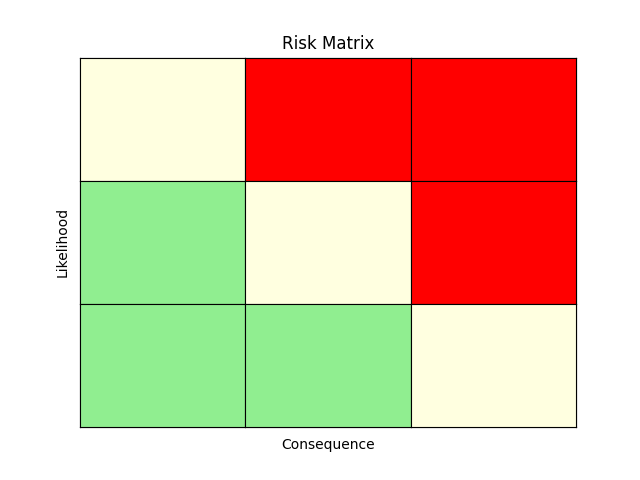
\includegraphics[width=12cm]{pictures/rm_template.png}
  \caption{Possible risk matrix, generated from the RMF.}
  \label{fig:rm_template}
\end{figure}

As next, the logged values are presented to show the raw data which the following example shows:

\begin{lstlisting}
INFO - root - 07/19/2022 05:01:32 PM: Current memory usage: 431.062129MB; Peak memory usage: 1279.472193MB
INFO - root - 07/19/2022 05:01:33 PM: Device 0: b'NVIDIA GeForce RTX 3060 Ti', Memory : (1.50% free): 8589.934592(total), 128774144 (free), 8461.160448 (used)
INFO - root - 07/19/2022 05:01:33 PM: Time to execute the attack: 176.75
\end{lstlisting}
